\documentclass{article}
\usepackage[utf8]{inputenc}
\usepackage{graphicx}
\usepackage{subfigure}
\usepackage{float}
\usepackage{indentfirst}
\usepackage{caption}
\usepackage{subcaption}
\usepackage[a4paper,includeheadfoot,margin=3cm]{geometry}
\usepackage{amsmath}
\usepackage[subrefformat=parens,labelformat=parens]{subfig}
%\titleformat{\subsection}{\normalsize}%{}{0em}{}

\title{DD2423 - Image Analysis and Computer Vision\\
  \large Lab 1}
\author{
  Gabriela Zarzar Gandler\\
  \texttt{gzrsm@kth.se}
  \and
 Huijie Wang\\
  \texttt{huijiew@kth.se}
}
\date{November 2016}

\begin{document}

\maketitle

\section{Fourier Transform}
\begin{enumerate}

%Q1
\item \textbf{Repeat this exercise with the coordinates $p$ and $q$ set to $(5, 9), (9, 5), (17, 9), (17, 121), (5, 1)$ and $(125, 1)$ respectively. What do you observe?}

As shown in Figure. \ref{fig_pair1}, \ref{fig_pair2} and \ref{fig_pair3} ,we can find that  $(5, 9)$ and $(9, 5)$ are mirrored by diagonal, and $(17, 9)$ and $(17, 121)$ , $(5, 1)$ and $(125, 1)$ are mirrored by y-axis and x-axis respectively. 
As a result, the wavelength is the same for each pair. We observe that, since the representation in the frequency domain is non-zero in one point only, a unique sinusoid with this frequency is obtained by calculating the inverse Fourier transform.

\begin{figure}[H]
    \centering
    \subfigure{
        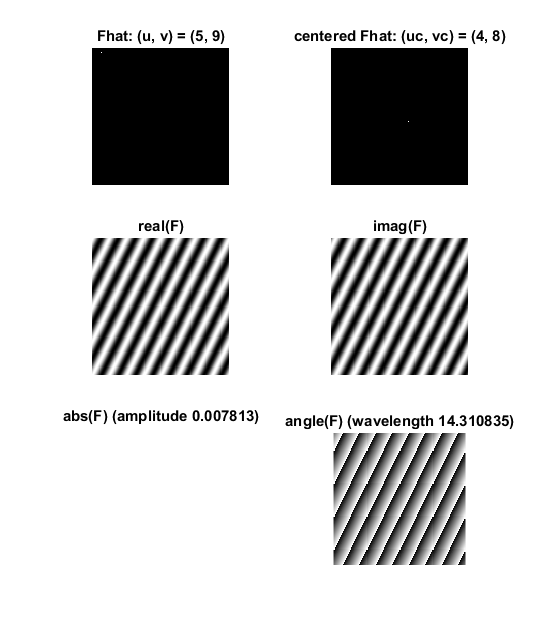
\includegraphics[height =8cm]{Lab1_1_3_Q1_fig1.png}
        }
    \subfigure{
        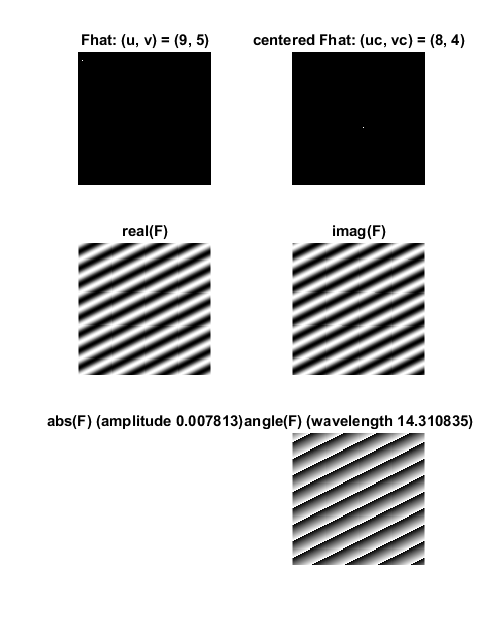
\includegraphics[height=8cm]{Lab1_1_3_Q1_fig2.png}
        }
    \caption{$p,q = (5, 9) \& (9,5)$}
    \label{fig_pair1}
\end{figure}

\begin{figure}[H]
    \centering
    \subfigure{
        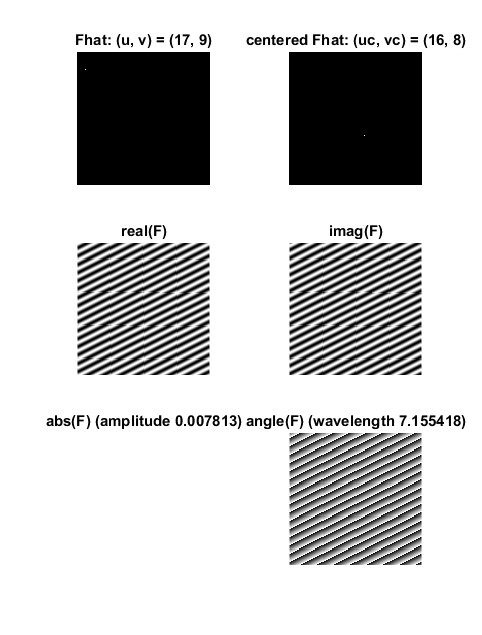
\includegraphics[height =8cm \linewidth]{Lab1_1_3_Q1_fig3.png}
        }
    \subfigure{
        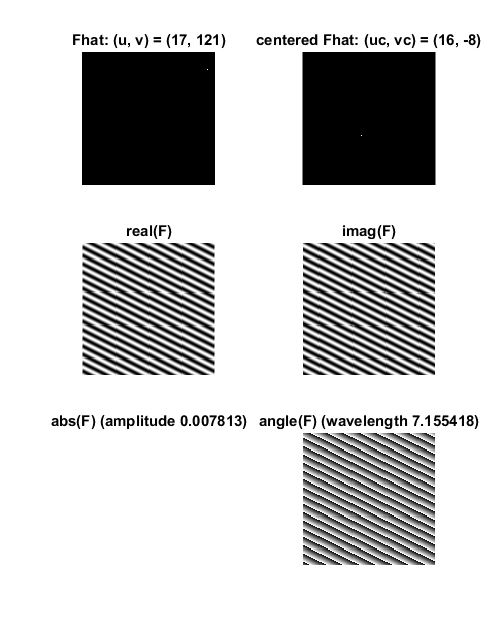
\includegraphics[height =8cm]{Lab1_1_3_Q1_fig4.png}
        }
    \caption{$p,q = (17, 9) \& (17,121)$}
    \label{fig_pair2}
\end{figure}

\begin{figure}[H]
    \centering
    \subfigure{
        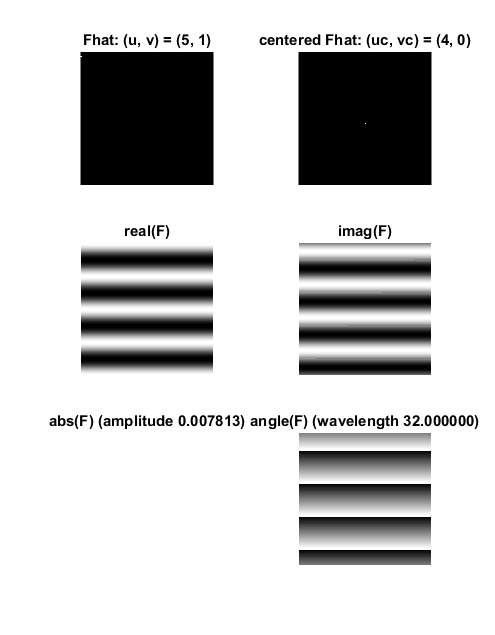
\includegraphics[height =8cm]{Lab1_1_3_Q1_fig5.png}
        }
    \subfigure{
        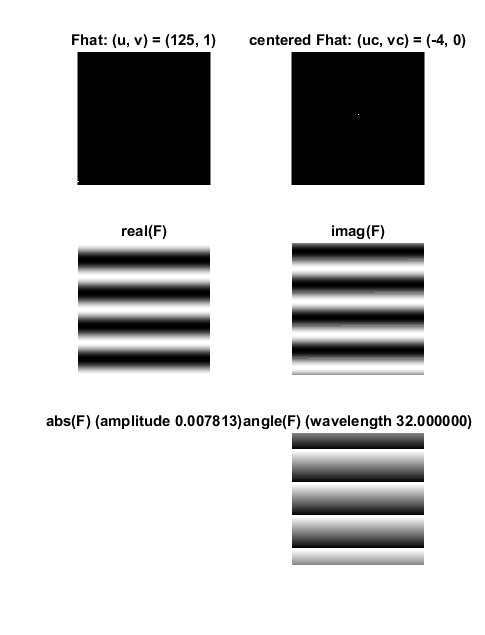
\includegraphics[height =8cm]{Lab1_1_3_Q1_fig6.png}
        }
    \caption{$p,q = (5, 1) \& (125,1)$}
    \label{fig_pair3}
\end{figure}

%Q2
\item \textbf{Explain how a position $(p, q)$ in the Fourier domain will be projected as a sine wave in the spatial domain. Illustrate with a \textsc{Matlab} figure.}

Figure. \ref{fig_sine} is an example of Sine wave in the spatial domain with respect to the frequency representation with the only non-zero coordinate $(125,1)$. Since there is only one element in the frequency spectrum which is non-zero, the signal is represented by one single component. The sine wave emerges from the complex exponential term in the expression of the inverse Fourier transform. Then the amplitude doesn't change in the graph. The angular frequency of the signal is determined by the only white point in Fhat. 

\begin{figure}[H]
    \centering
    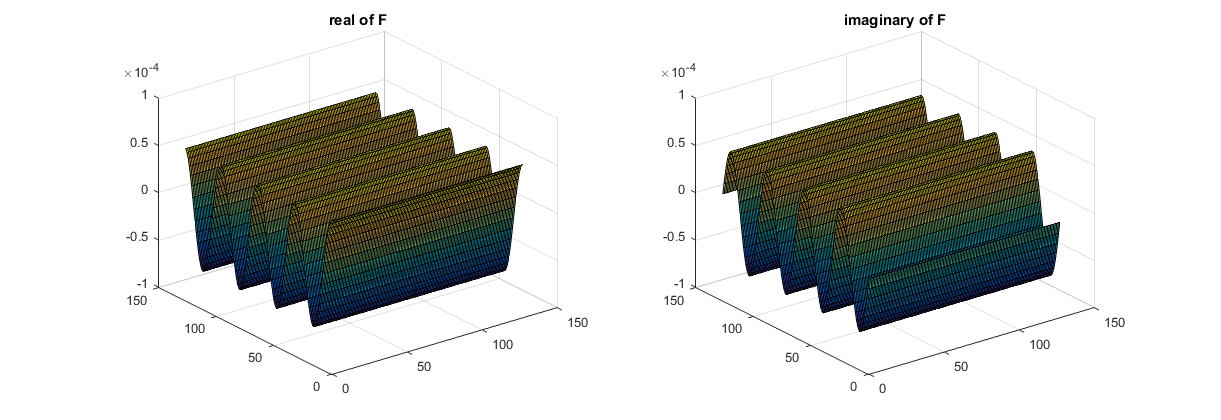
\includegraphics[width =  \linewidth]{Lab1_1-3_Q2_fig.png}
    \caption{Sine wave in the spatial domain for the representation with the only non-zero coordinate $(125,1)$ in Fourier Domain}
    \label{fig_sine}
\end{figure}

%Q3
\item \textbf{How large is the amplitude? Write down the expression derived from Equation (4) in these notes. Complement the code (variable amplitude) accordingly.}

We will calculate the amplitude of the sinusoid, by taking the frequency representation that has the point $(5,9)$ as the only non-zero (1) pixel:

\begin{align*}
    F(x) = \frac{1}{N}\sum_{u\in[0,...,N-1]^2}^{} \hat F(u) e^{\frac{2\pi i u^T x}{N}} \\
    = \frac{1}{N} \hat F((5,9)) e^{\frac{2\pi i (5,9)^T x}{N}} \\
    = \frac{1}{N} \times 1 \times (\cos{\frac{2\pi (5,9)^T x}{N}} + i \sin{\frac{2\pi (5,9)^T x}{N}}) \\
    = \frac{\cos{\frac{2\pi (5,9)^T x}{N}}}{N} + i \frac{\sin{\frac{2\pi (5,9)^T x}{N}}}{N}
\end{align*}

Therefore the amplitude can be written as:

\begin{align*}
    |F(x)| = \sqrt{\frac{\cos{\frac{2\pi (5,9)^T x}{N}}^2}{N^2} + \frac{\sin{\frac{2\pi (5,9)^T x}{N}}^2}{N^2}} = \sqrt{\frac{1}{N^2}} = \frac{1}{N} = \frac{1}{128}
\end{align*}

%Q4
\item \textbf{How does the direction and length of the sine wave depend on $p$ and $q$? Draw an illustrative figure on paper. Write down the explicit expression that can be found in the lecture notes. Complement the code (variable wavelength) accordingly.}
\par
The direction can be explained by the centralized (shifted version) $p$ and $q$. In the code they are represented by $uc$ and $vc$. This makes sense intuitively as well, as pictured in Figure \ref{fig:direction}.

\begin{figure}[H]
    \centering
    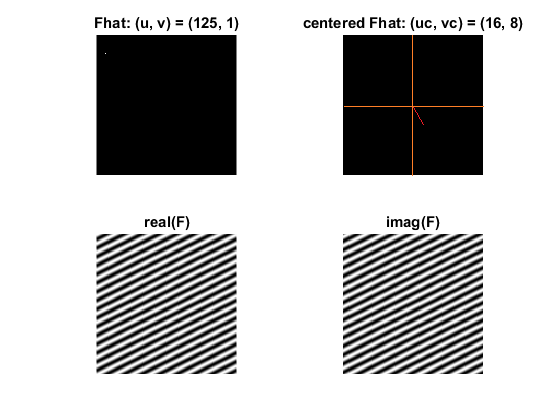
\includegraphics[width = 0.7 \linewidth]{direction.png}
    \caption{Illustration of direction of the sine wave}
    \label{fig:direction}
\end{figure}

% [Attention]Here I am skipping these, please check whether there's any part you wanna keep, Gabi:) - Huijie

%Write down how this direction depends on $p$ and $q$. The direction is simply the direction of the arrow, which makes sense intuitively.
%Draw the arrow

%Write down the expression of the length:
%wavelength = sz/sqrt(power(uc,2) + power(vc,2)); show the same expression, but depending on p and q
%In the figure of point (5,1) or (125,1) it is possible to notice the wavelength just by looking at the graphs of real(F) and imag(F). The wavelengths in this case are the same for (5,1) and (125,1).
%Huijie, I think this expression you wrote below is for uc and vc, instead of p and q
% True!!!!
\begin{align}
    \omega = (\omega_1, \omega_2) = (2\pi\frac{uc}{M},2\pi\frac{vc}{N})) ;\\
    wavelength = \frac{2\pi}{\sqrt{{\omega_1}^2 + {\omega_2}^2}}\\
     = \frac{2\pi}{\sqrt{(\frac{2\pi uc}{M})^2 + (\frac{2\pi vc}{N})^2}}
\end{align}
, in the case $M = N$, we get $wavelength = \frac{N}{\sqrt{uc^2 + vc^2}}$.
According to expression in Matlab, $uc = p-1$ in the case $p$ is equal or smaller than $sz$, the size of the image, and $uc = p-1 -sz$ in the case $p$ is larger than $sz$. And the same for the relation between $vc$ and $q$.

%Q5
\item \textbf{What happens when we pass the point in the center and either $p$ or $q$ exceeds half the image size? Explain and illustrate graphically with \textsc{Matlab}!}

%Periodicity 
\par
The representation can be seen as a periodic function that keeps repeating in all directions. So we can shift the coordinates so that the center represents lower frequencies, while the borders represent higher frequencies, as shown in Figure \ref{fig:fftshift}.
\par
This shifting means that the quadrants of the representation swap places. 
For example, the point (125,1) is beyond half the image size and it is symmetrical to the point (5,1). This means that in the centered representation these vectors are the same, but with opposite direction. So these points actually represent the same patterns, but in the opposite direction.This can be seen in Figure \ref{fig_pair3}. We can also regard this shifting as a change in the interval of the period, for example, from $(0,2\pi)$ to $(-\pi, \pi)$ in both dimension of Fourier domain.

\begin{figure}[H]
    \centering
    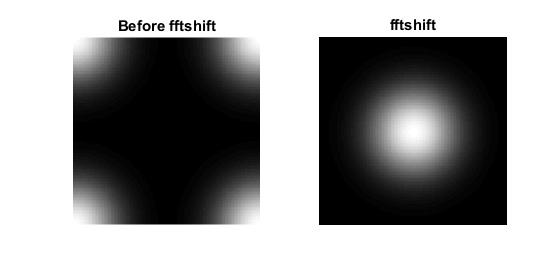
\includegraphics[width = 0.7 \linewidth]{Lab1_1-3_Q5_fftshift.png}
    \caption{Illustration of fuction \textbf{fftshift}}
    \label{fig:fftshift}
\end{figure}




%Q6
\item \textbf{What is the purpose of the instructions following the question ``What is done by these instructions?'' in the code?}

Firstly, in Fourier Domain, the discrete index of $x$ starts from 0 instead of 1, the default initial index in Matlab. So first 1 is subtracted from the index. Secondly, as in Matlab the center is regarded as the corner of the picture, by subtracting the size of the image we can turn the origin of coordinates into the center. 

%Q7
\item \textbf{Why are these Fourier spectra concentrated to the borders of the images? Can you give a mathematical interpretation? Hint: think of the frequencies in the source image and consider the resulting image as a Fourier transform applied to a 2D function. It might be easier to analyze each dimension separately!}
\par

Figure \ref{fig1.4} shows the log-magnitude in the Fourier domain, for the functions $F$, $G$ and $H$.
 Take the example of $F$, mathematically, the transformation is shown as following:\\


\begin{figure}[H]
        \centering
        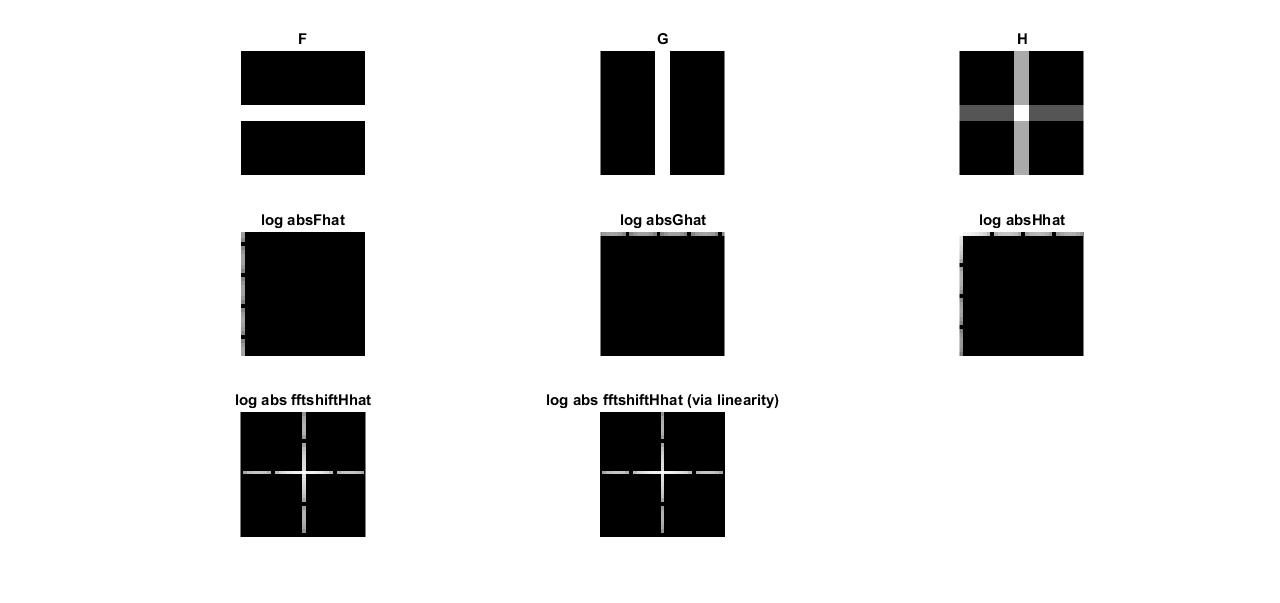
\includegraphics[width=16cm]{14(zoomed2).jpg}
        \caption{Analysis of the logarithm of Fourier spectra (zoomed in for easier interpretation)}
        \label{fig1.4}
\end{figure}

For any point $(u,v)$ in Fourier Domain,

\begin{align*}
    \hat f(u,v) = \frac{1}{\sqrt{MN}} \sum_{m = 0}^{M-1} \sum_{n = 0}^{N-1} f(m,n) e^{-2\pi i \frac{mu}{M}} e^{-2\pi i \frac{nv}{N}}\\
    = \frac{1}{\sqrt{N}} \sum_{n = 0}^{N-1} (\frac{1}{\sqrt{M}} \sum_{m = 0}^{M-1} f(m,n) e^{-2\pi i \frac{mu}{M}}) e^{-2\pi i \frac{nv}{N}}
\end{align*}
As there is only changes of frequences vertically, the term $\frac{1}{\sqrt{M}} \sum_{m = 0}^{M-1} f(m,n) e^{-2\pi i \frac{mu}{M}}$ is only dependent on $m$. Furthermore, for any n, $f(m,n) = 1$ in the range $m = (56,71)$ (in image $F$), and  $f(m,n) = 0$ otherwise.  So we can pull out this term and only keep the terms where $f(m,n) = 1$. So that we get:
\begin{align*}
    \hat f(u,v) = (\frac{1}{\sqrt{N}} \sum_{n = 0}^{N-1} e^{-2\pi i \frac{nv}{N}})
    (\frac{1}{\sqrt{M}} \sum_{m = 56}^{71} e^{-2\pi i \frac{mu}{M}}))
\end{align*}
Now we can find that the second term is some number dependent on $u$, while the first term is a \textbf{delta function} about $v$, which always equals $0$ when $v>0$ and equals to $\frac{1}{\sqrt{N}} \sum_{n = 0}^{N-1} 1 = \frac{N}{\sqrt{N}}$ when $v=0$. %That is because  $\frac{1}{\sqrt{N}} \sum_{n = 0}^{N-1} e^{-2\pi i \frac{nv}{N}}$ contains $v$ whole periods of wave and cancel out each other when $v>0$. 
As it can be seen, these Fourier spectra concentrate to the borders of the images (where $v = 0$).

%Q8
\item \textbf{Why is the logarithm function applied?}

The logarithm function is applied because originally the range of the values of the Fourier spectra (i.e. the intensity values in the Fourier image) is too large to be displayed on the screen. In the original spectra it is only possible to target the points with highest magnitude, i.e. the points that represent the lowest frequencies. By applying the log function other frequencies become visible as well.

%Q9
\item \textbf{What conclusions can be drawn regarding linearity? From your observations
can you derive a mathematical expression in the general case?}
\par
As shown in Figure \ref{fig1.4}, the result of \textbf{Hhat} is exactly the same as the sum of \textbf{Fhat} with $2 \times $ \textbf{Ghat}. Thus, we can conclude that:
$$F[a f_1(m,n) + b f_2(m,n)] = a \hat f_1(u,v) + b \hat f_2(u,v)$$

for $f_1$ and $f_2$ representations in the spatial domain, $\hat f_1$ and $\hat f_2$ their Fourier transforms and $a$ and $b$ constants.

%Q10
\item \textbf{Are there any other ways to compute the last image? Remember what multiplication in Fourier domain equals to in the spatial domain! Perform these alternative computations in practice.}
\par
A convolution in the Fourier domain equals to multiplication in the spatial domain. Therefore the Fourier transform of the multiplication $F \imes G$ can be simply replaced by the convolution of the Fourier transforms of F and G.

The Figure \ref{fig1.5} shows the log-magnitude of the Fourier transform of the image with the white square. It is possible to notice that the most representative frequencies lie on the main axis, as the transitions on the image are mainly vertical and horizontal. Finally the same graph is achieved via the convolution operation.

\begin{figure}[H]
        \centering
        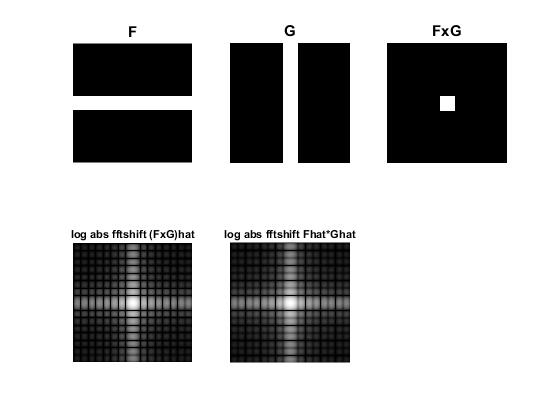
\includegraphics[width=11cm]{15.jpg}
        \caption{Convolution in the frequency domain and multiplication in the spatial domain}
        \label{fig1.5}
\end{figure}

Additionally a convolution in the spatial domain is equivalent to a multiplication in the Fourier domain. We tested this as well and the result (zoomed in for better visualization) can be seen in Figure \ref{fig1.52}. The third image in Figure \ref{fig1.52} displays multiplication in the frequency domain, while the fifth image displays the convolution in the spatial domain. 

\begin{figure}[H]
        \centering
        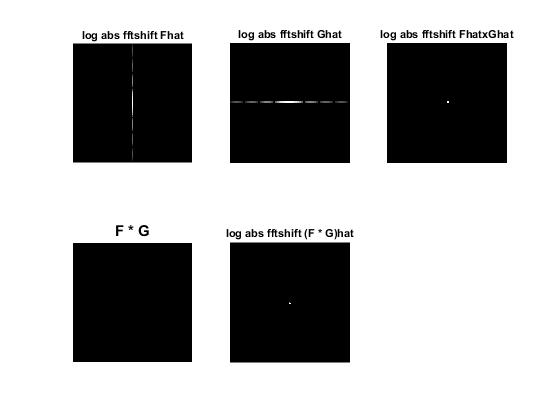
\includegraphics[width=11cm]{15(inverse).jpg}
        \caption{Multiplication in the frequency domain and convolution in the spatial domain}
        \label{fig1.52}
\end{figure}

%Q11
\item \textbf{What conclusions can be drawn from comparing the results with those in
the previous exercise? See how the source images have changed and analyze the effects
of scaling.}
\par
\begin{figure}[H]
        \centering
        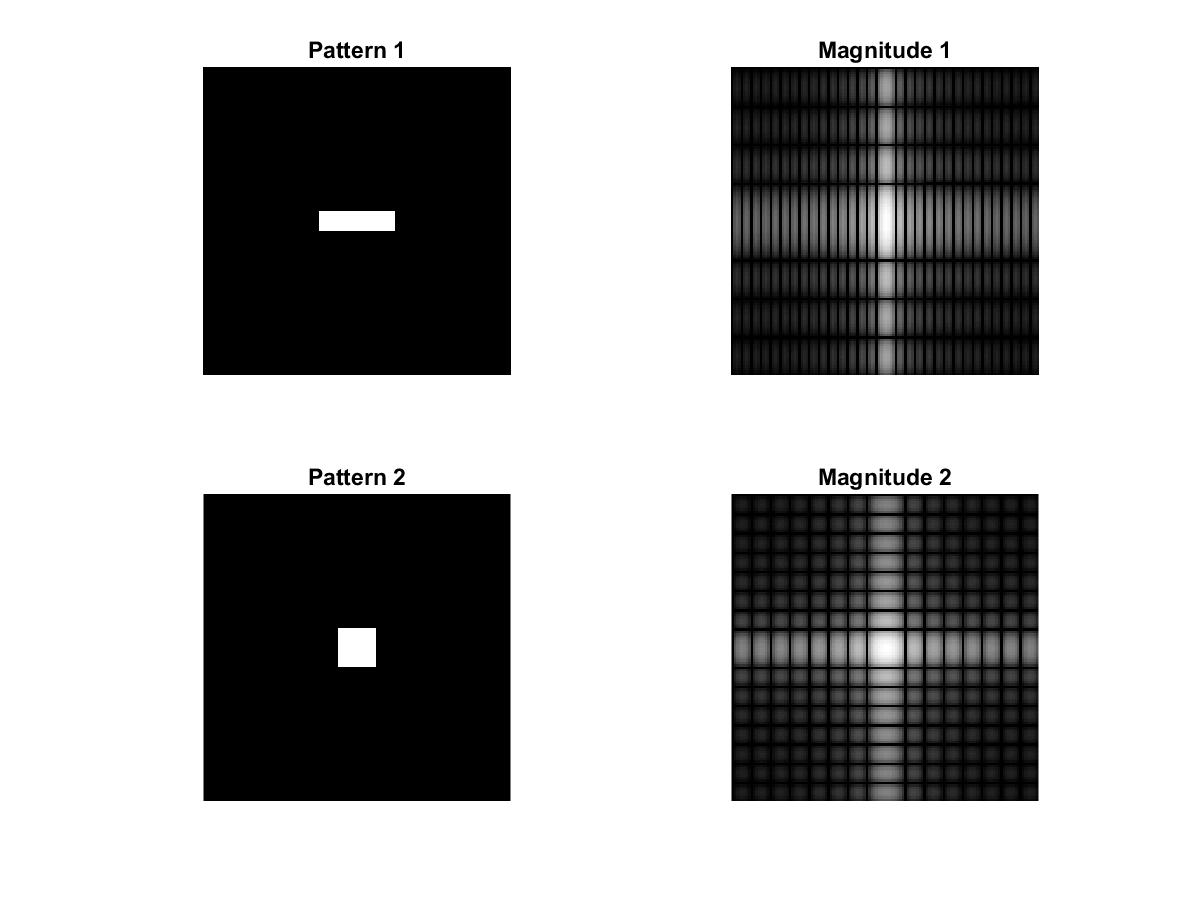
\includegraphics[width=10cm]{Lab1_1_6_Q11_fig.png}
        \caption{Scaling in different patterns}
        \label{fig1.6}
\end{figure}

As shown in Figure \ref{fig1.6}, in the second pattern, the square in the spatial domain is represented by the same frequency pattern in both x and y direction in Fourier domain. Compared to pattern 2, pattern 1 compresses along y-axis and expands along x-axis. As a result, the pattern in Fourier domain expands along y-axis and compresses along x-axis. 
We can conclude that the compression in one domain is an expansion in another, and vice versa. 

%Q12
\item \textbf{What can be said about possible similarities and differences? Hint: think of the frequencies and how they are affected by the rotation.}

A rotation in the spatial domain means the same rotation in the frequency domain, as shown in the Figure \ref{fig1.7}. This makes sense: as the directions of variations in the original image change, the representations of these variations in the frequency domain should also change accordingly.

Additionally we notice that the images with diagonal patterns have their frequency representations affected by discretization noise, as in Figure \ref{fig1.72}.

\begin{figure}[H]
        \centering
        \hspace{-1cm}
 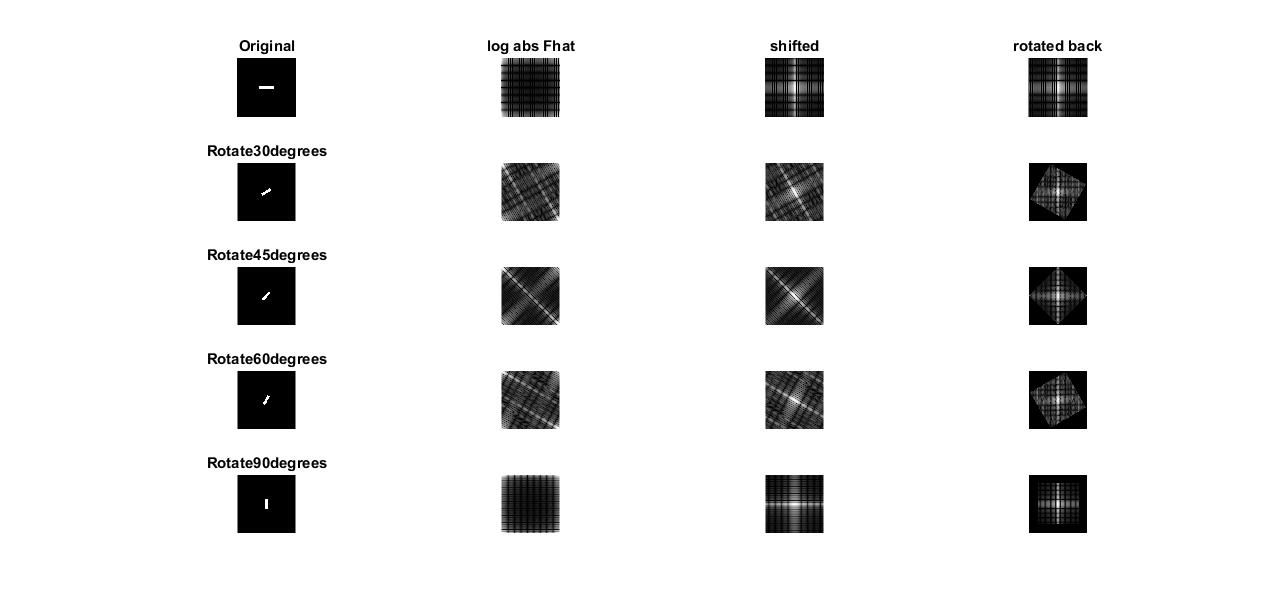
\includegraphics[width=18cm]{17.jpg}
        \caption{Rotation in spatial and frequency domains by different degrees}
        \label{fig1.7}
\end{figure}

\begin{figure}[H]
        \centering
        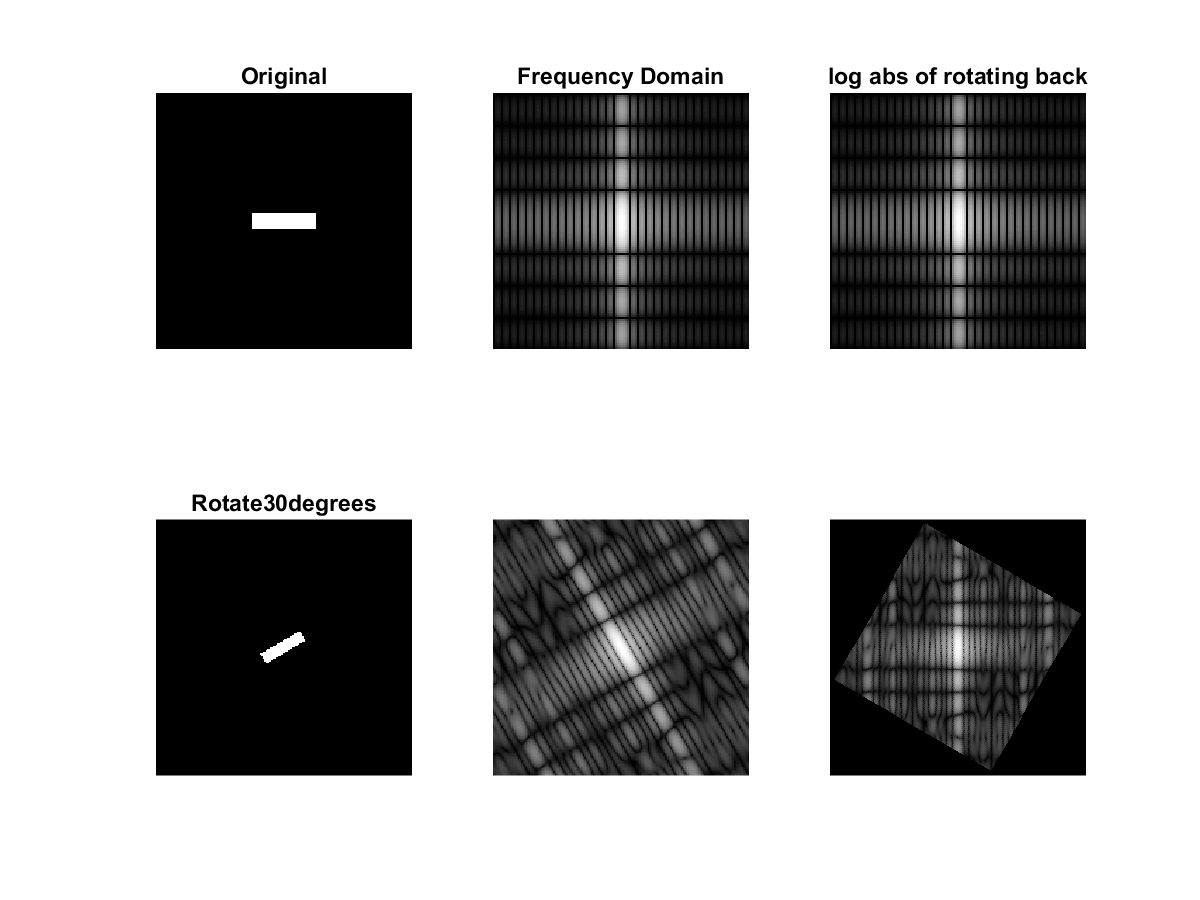
\includegraphics[width=12cm]{Lab1_1-7_Q12_fig2.png}
        \caption{Rotation and discretization noise}
        \label{fig1.72}
\end{figure}

%Q13
\\
\\
\newpage
\item \textbf{What information is contained in the phase and in the magnitude of the Fourier transform?}
\par
As it can be seen in Figure \ref{fig1.8}, by applying \textit{pow2image}, the information of magnitude is replaced and only information of phase is preserved. The displayed figure seems to be different, because the gray level values were affected. However all the objects in the image are properly represented when it comes to position in the image. Therefore we conclude that the phase keeps information regarding where the edges are located in the image, or where each frequency component is located.


On the other hand, by applying \textit{randphaseimage}, the information in the phase is randomized out so that only information of magnitude remains. This makes the resulting image so different, that it is not possible to recognize the original image anymore. This shows that the phase information is crucial to reconstruct the correct image in the spatial domain. The magnitude keeps the information about how much of a certain frequency component is present in the image. So this is kept even when the phase is randomized, but since the edges are not in the proper place, the resulting image still looks very different.

Figure \ref{fig1.82} shows an analysis on the original frequency spectrum.

\begin{figure}[H]
        \centering
        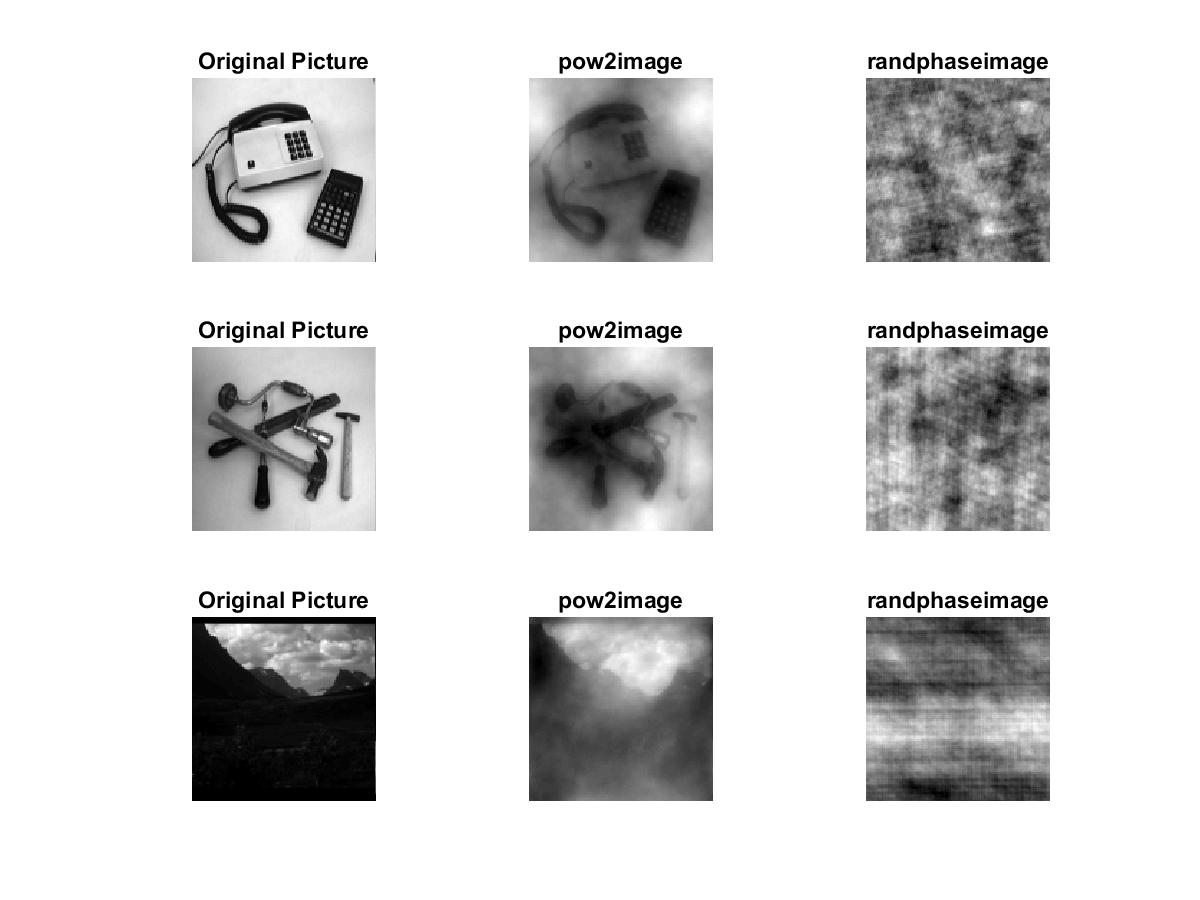
\includegraphics[width=15cm]{Lab1_1-8_Q13_fig.png}
        \caption{Figures with replaced magnitude and randomized phase}
        \label{fig1.8}
\end{figure}

\begin{figure}[H]
        \centering
        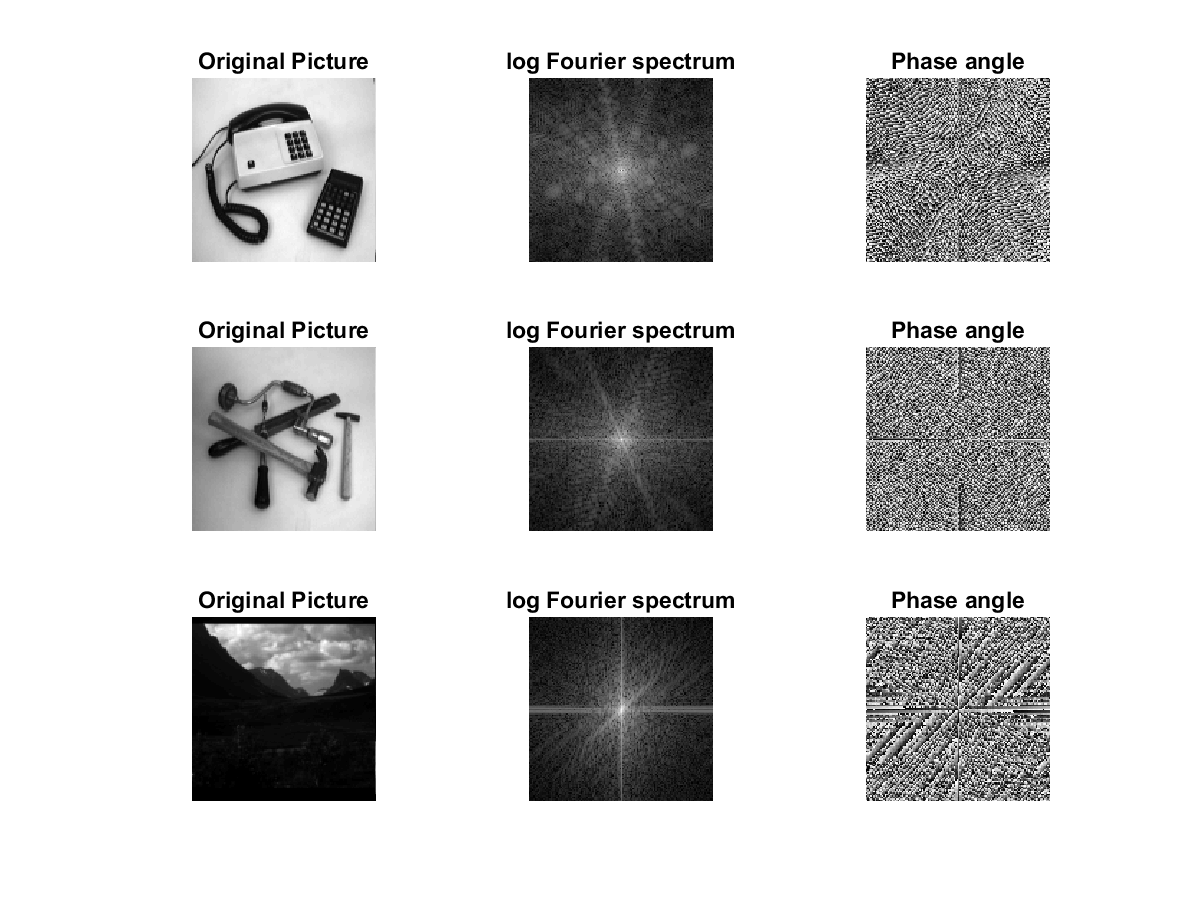
\includegraphics[width=15cm]{Lab1_1-8.png}
        \caption{Analysis of frequency spectrum}
        \label{fig1.82}
\end{figure}



\section{Gaussian convolution implemented via FFT}

\subsection{2.3 Filtering procedure}
\item \textbf{Show the impulse response and variance for the above mentioned t-values. What are the variances of your discretized Gaussian kernel for t = 0.1, 0.3, 1.0, 10.0 and 100.0?}

%The Gaussian outputs a `weighted average' of each pixel's neighborhood, with the average weighted more towards the value of the central pixels. This is in contrast to the mean filter's uniformly weighted average. Because of this, a Gaussian provides gentler smoothing and preserves edges better than a similarly sized mean filter.

%One of the principle justifications for using the Gaussian as a smoothing filter is due to its frequency response

%Both filters attenuate high frequencies more than low frequencies, but the mean filter exhibits oscillations in its frequency response. The Gaussian on the other hand shows no oscillations. In fact, the shape of the frequency response curve is itself (half a) Gaussian. So by choosing an appropriately sized Gaussian filter we can be fairly confident about what range of spatial frequencies are still present in the image after filtering, which is not the case of the mean filter. 

The result of the convolution of the Gaussian kernel with the impulse function is shown in Figure \ref{fig222} for the five variance values, in the middle column. The kernel itself can be seen in the first column, while the last column displays the convolution via discgaussfft. As expected, the three columns display the same pattern for every row. Figure \ref{fig2.1} shows the result of the convolution in more detail. The calculated covariances of the Gaussian output, for the above mentioned t values were:

for t = 0.1:
\newline
   0.013296725185226   0.000000000000020
\newline
   0.000000000000020   0.013296725185592
\newline
for t = 0.3:
\newline
   0.281053830089380   0.000000000000002
\newline
   0.000000000000002   0.281053830089784
\newline
for t = 1:
\newline
   0.999999788773478   0.000000000000002
\newline
   0.000000000000002   0.999999788773594
\newline
for t = 10:
\newline
  10.000000000001283   0.000000000000001
\newline
   0.000000000000001  10.000000000001380
\newline
for t = 100
\newline
  99.999999328229492   0.000000000000000
\newline
0.000000000000000  99.999999328229904
   
%variance = 0.1

%ans =

%    0.0133    0.0000\\
%    0.0000    0.0133

%variance = 0.3

%ans =

%    0.2811    0.0000\\
%    0.0000    0.2811

%variance = 1

%ans =

%    1.0000    0.0000\\
%    0.0000    1.0000

%variance = 10

%ans =

%   10.0000    0.0000\\
%    0.0000   10.0000

%variance = 100

%ans =

%  100.0000    0.0000\\
%    0.0000  100.0000
    
%\textbf{Why for $t = 0.1 , 0.3$ it doesn't work?????}
    
\begin{figure}[H]
        \centering
        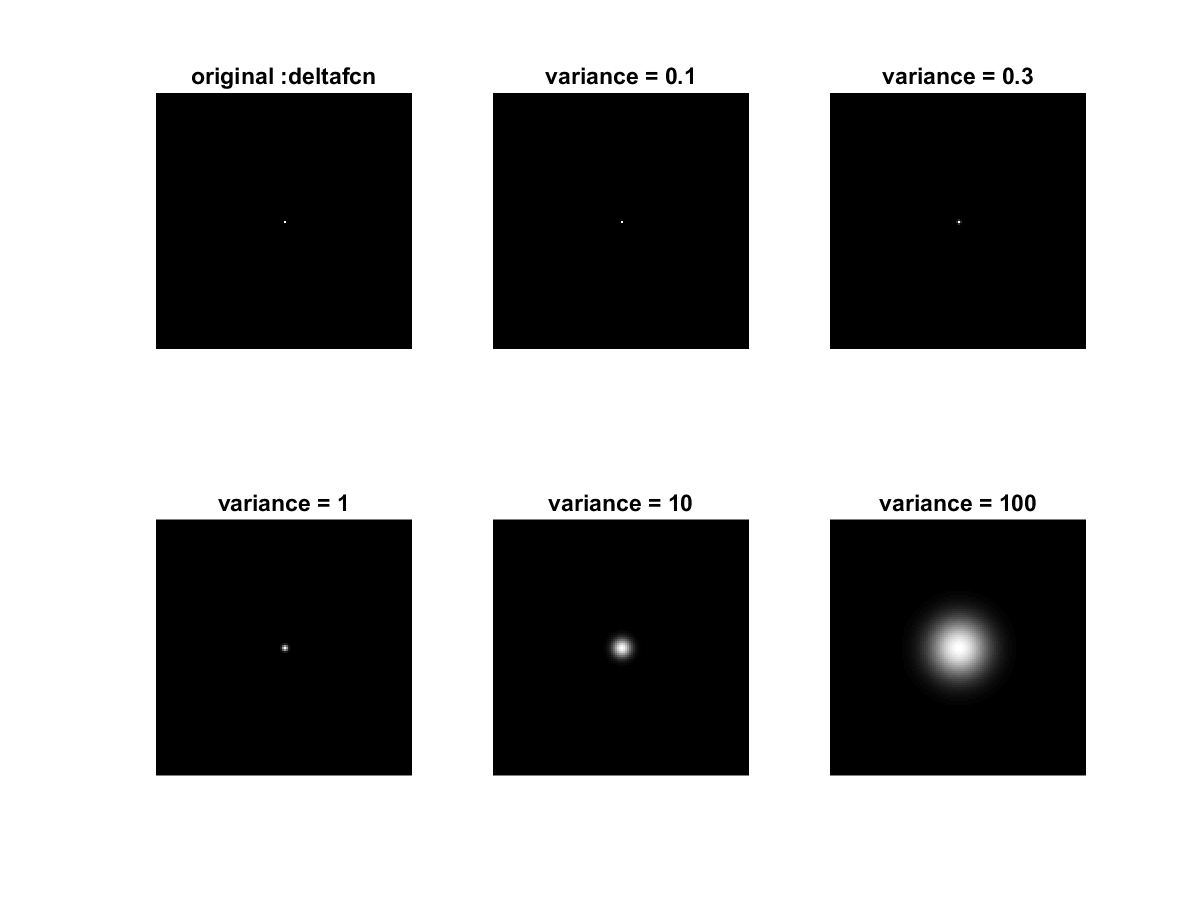
\includegraphics[width=15cm]{Lab1_2-1_Q14_fig.png}
        \caption{Applying Gaussian Filters with different variances}
        \label{fig2.1}
\end{figure}

\begin{figure}[H]
        \centering
        \hspace{-2cm}
        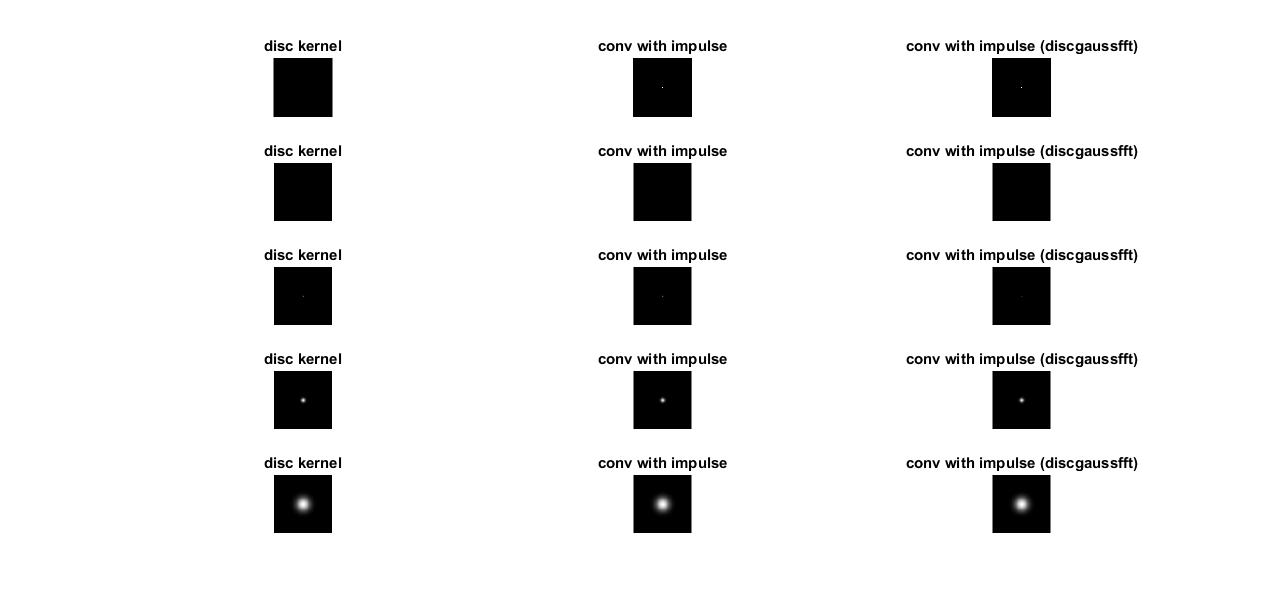
\includegraphics[width=18cm]{214comp.png}
        \caption{Comparing discrete Gaussian kernel with output from convolution of kernel with impulse function, for difference variance values}
        \label{fig222}
\end{figure}

\item \textbf{Are the results different from or similar to the estimated variance? How
does the result correspond to the ideal continuous case? Lead: think of the relation
between spatial and Fourier domains for different values of t.}

The variances are close to the ideal continuous case, but not exactly the same. 
This is due to the fact that discretization noise is more significant for lower frequencies. For example, when variance equals 0.1, the density of the sampled Gaussian is concentrated within a small part around the origin, which means that Gaussian is not properly described by the sampling. We can also notice that when the variance continuously grows it will also be less accurately represented by the discretized kernel. That is because we sample the Gaussian filter within a specific range that becomes insufficient to represent all the variance of the Gaussian, which leads to a lose of high frequency information (at the tail part of Gaussian) in Fourier domain. In this case we can obviously observe the effect when variance is larger than 256. Therefore an intermediate value for the variance needs to be used so that the result gets close to the ideal continuous case.
%Higher variances tend to output more accurate values than lower variances.

%This is due to the fact that discretization noise is more significant for lower frequencies?

%Similar when $t>=1$ and different when $t<1$

\begin{figure}[H]
        \centering
        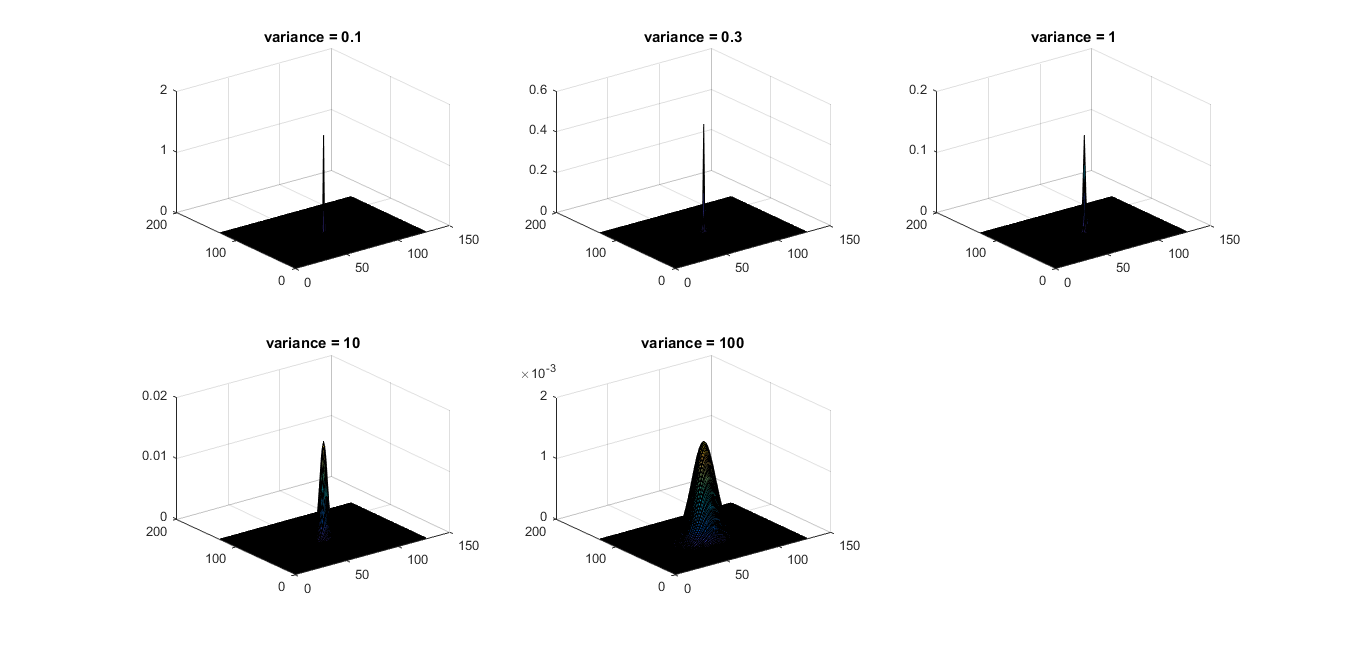
\includegraphics[width=15cm]{Lab1_2-1_Q15_fig.png}
        \caption{Sampled Gaussion filters with different variances}
        \label{fig2.1-2}
\end{figure}

%Q16
\item \textbf{Convolve a couple of images with Gaussian functions of different variances
(like t = 1.0, 4.0, 16.0, 64.0 and 256.0) and present your results. What effects can you
observe?}

Figures \ref{fig2161}, \ref{fig2162} and \ref{fig2163} display results of convolutions with Gaussian kernel of increasing variance. It can be noticed that, as the variance increases, the blurring increases as well.

\begin{figure}[H]
        \centering
        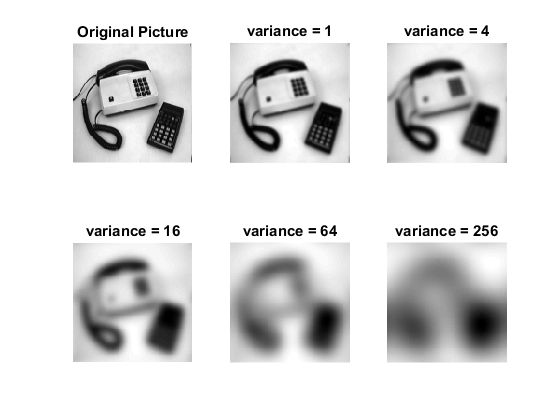
\includegraphics[width=10cm]{16blur1.png}
        \caption{Convolution of image with Gaussian kernel of different variances}
        \label{fig2161}
\end{figure}

\begin{figure}[H]
        \centering
        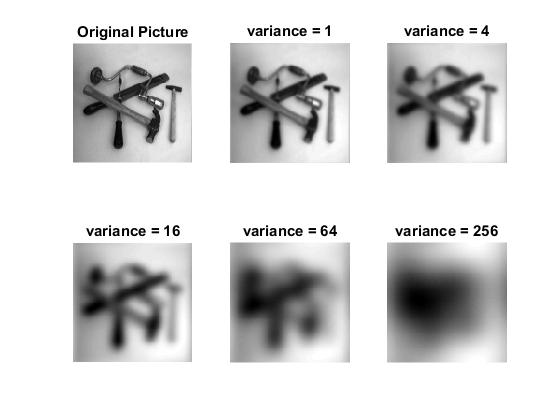
\includegraphics[width=10cm]{16blur2.png}
        \caption{Convolution of image with Gaussian kernel of different variances}
        \label{fig2162}
\end{figure}

\begin{figure}[H]
        \centering
        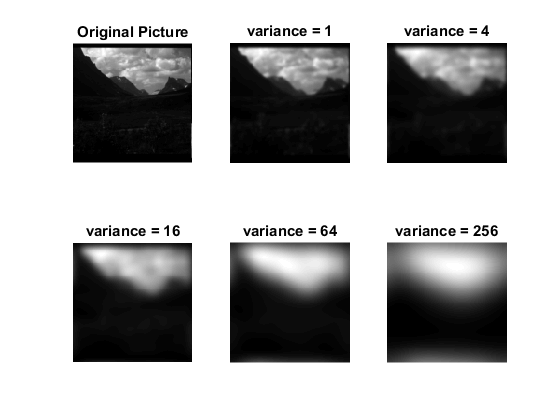
\includegraphics[width=10cm]{16blur3.png}
        \caption{Convolution of image with Gaussian kernel of different variances}
        \label{fig2163}
\end{figure}

\section{Smoothing}

\item \textbf{What are the positive and negative effects for each type of filter? Describe what you observe and name the effects that you recognize. How do the results depend on the filter parameters? Illustrate with Matlab Figure(s).}

Gaussian noise is a kind of noise that affects all pixels of the image. It simply adds a random Gaussian-distributed uncorrelated noise to every pixel, with mean zero and manually set standard deviation.

The salt and pepper noise affects specific pixels of the image, which are randomly picked. The number of affected pixels is determined by a fraction set by the user. Half of these noisy pixels will be white, while the other half is black.

For the smoothing of the Gaussian noise, we reached the following conclusions:

- The gaussian filter helps to attenuate the effect of the noise, but it also negatively affects the edges in the image, which becomes blurred. The higher the variance, the more blurred the image;

- The median filter is not so appropriate, because it gives a painting effect to the image. The higher the window size, the stronger the painting effect;

- The ideal low-pass filter is tricky to use, because it introduces ringing for some cut-off frequencies. By setting a cut-off frequency that avoids the ringing effect and attenuates the gaussian noise (around $0.22$ cycles per pixel), we get a more visually pleasing image, but the noise is still present.

For the smoothing of the salt and pepper noise, we reached the following conclusions:

- The gaussian filter spreads the salt and pepper noise, blurring the inconvenient dots, but leaving their ``marks'';

- The median filter is the best one to correct salt and pepper noise, because it results in quite clear images, without affecting the other properties so much;

- Finally the ideal low-pass filter deletes the punctual salt and pepper marks, but also creates a strange coarse texture out of the blurring.

\begin{figure}[H]
    \centering
    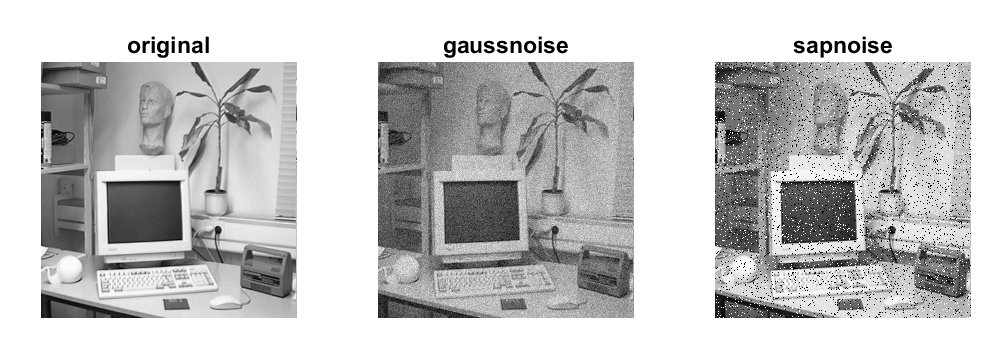
\includegraphics[width = \linewidth]{Lab1_3-1_Q17_fig1_original.png}
    \caption{Original Picture adding Gaussian noise and SAP noise}
    \label{figOrg}
\end{figure}

\begin{figure}[H]
    \centering
    \subfloat[Gaussian Filter]{
        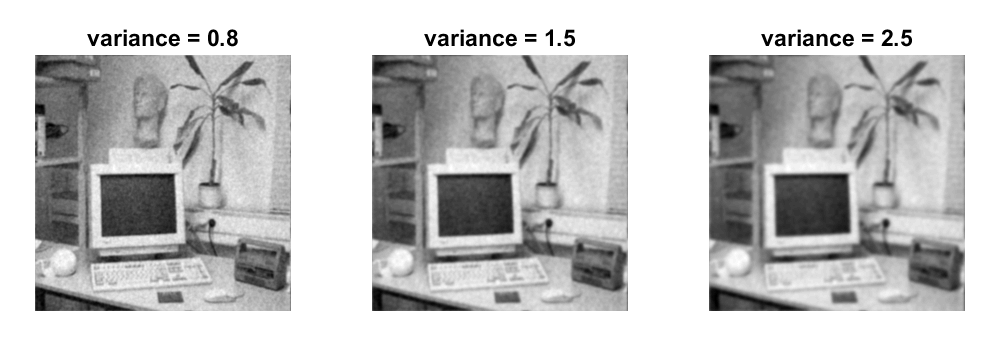
\includegraphics[width = \linewidth]{Lab1_3-1_Q17_fig2_GaussNoise_GaussF.png}
        %\subcaption{Gaussian Filter}
        \label{figGN_GF}
        }\\
    \subfloat[Median Filter]{
        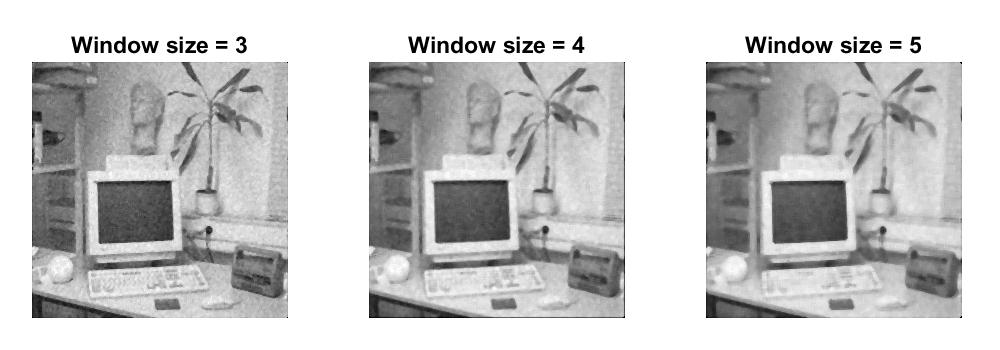
\includegraphics[width = \linewidth]{Lab1_3-1_Q17_fig2_GaussNoise_MedianF.png}
        %\subcaption{Median Filter}
        \label{figGN_MF}
        }\\
    \subfloat[Ideal Low-pass Filter]{
        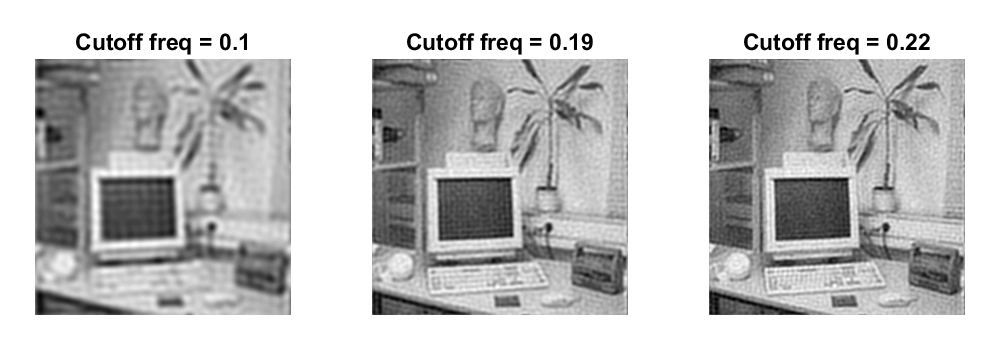
\includegraphics[width = \linewidth]{Lab1_3-1_Q17_fig2_GaussNoise_IdealF.png}
        %\subcaption{Ideal Low-pass Filter}
        \label{figGN_IF}
        }\\
    \caption{Smoothing for Gaussian Noise through different filters with different parameters}
    \label{figGN}
\end{figure}


\begin{figure}[H]
    \centering
    \subfloat[Gaussian Filter]{
        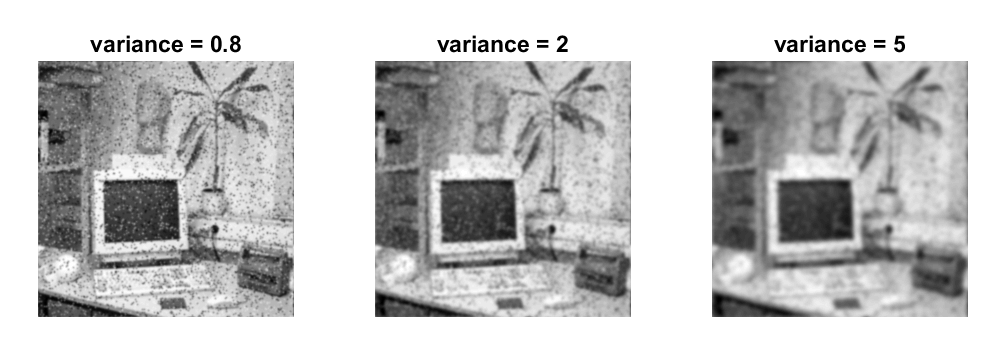
\includegraphics[width = \linewidth]{Lab1_3-1_Q17_fig3_SAPNoise_GaussF.png}
        %\subcaption{Gaussian Filter}
        \label{figSAPN_GF}
        }\\
    \subfloat[Median Filter]{
        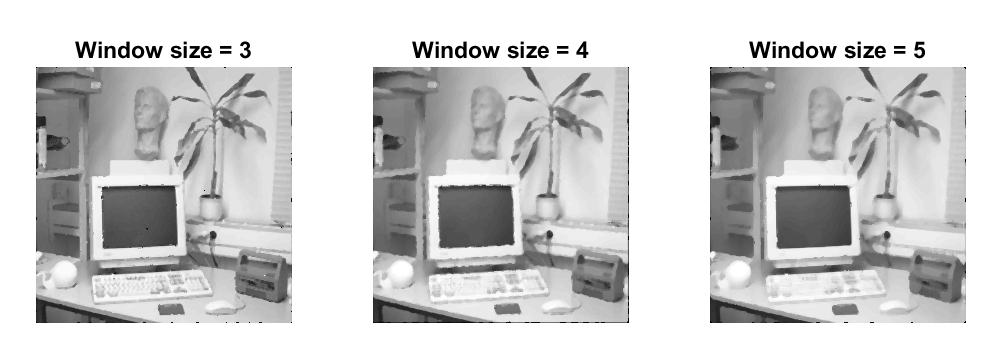
\includegraphics[width = \linewidth]{Lab1_3-1_Q17_fig3_SAPNoise_MedianF.png}
        %\subcaption{Median Filter}
        \label{figSAPN_MF}
        }\\
    \subfloat[Ideal Low-pass Filter]{
        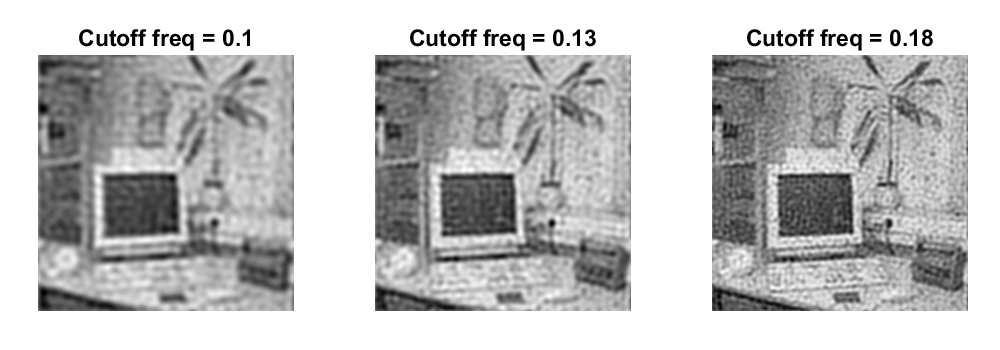
\includegraphics[width = \linewidth]{Lab1_3-1_Q17_fig3_SAPNoise_IdealF.png}
        %\subcaption{Ideal Low-pass Filter}
        \label{figSAPN_IF}
        }\\
    \caption{Smoothing for SAP Noise through different filters with different parameters}
    \label{figSAPN}
\end{figure}

\item \textbf{What conclusions can you draw from comparing the results of the respective methods? Can you give a mathematical interpretation to explain the effects of each filter?}

Gaussian filter applies a discretized convolution to the image, which means that each pixel becomes a weighted average of its neighbouring pixels. The closer a pixel is from the origin of the filter, the more important it is in the weighted average. This means that gaussian filters, differently from average filters, treat the neighbouring pixels differently. The parameter determines how spread this filter is, which affects the amount of blurring effect in the image. This can be noticed in the pictures, as the gaussian smoothing averages all the information around. Since the Gaussian filter is represented by a Gaussian in both spatial and frequency domains, it is a non-negative and non-oscillatory filter, hence it causes no ringing in the spatial domain.

Median filter takes the intensity values of the neighbouring pixels and ranks them. Then it updates the value of the corresponding pixel by setting its value as the median intensity in the ranked list. This is a perfect approach to attenuate salt and pepper disturbations. Since the salt and pepper noise is either white or black (it lies on either one of the extreme ends of the gray level scale) and since the affected pixels are selected randomly, the noisy pixels will seldom be median of the ranked list of pixels. Increasing the fraction of noisy pixels also increases the chance of it happening, though. But for a general case the filter is able to ``clean''the image from salt and pepper, without affecting much of other properties in the image, such as edges.

Finally the ideal low-pass filter is a filter that affects the signal via its frequency domain, by means of thresholding the frequencies. This happens by multiplying the frequency spectrum of the image by a modulation transfer function, which cancels out frequencies that are beyond a certain distance from the origin. This causes noise filtering, as we can perceive in the pictures, but it also causes some side-effects, as the existence of ringing. Ringing is an artifact present in the spatial domain, characterized by oscillations around edges. This artifact is traded off with desired frequency domain characteristics. The desired frequency response may cause ringing, while reducing or eliminating ringing may worsen the frequency response. This phenomenon shows how a filter which is ideal in the frequency domain may not be ideal in the spatial domain. Finally, the oscillations themselves are a result of the sinc function, which is the representation of the modulation transfer function (the brick-wall filter) in the spatial domain.

% Explain ringing!
\item \textbf{What effects do you observe when subsampling the original image and the smoothed variants? Illustrate both filters with the best results found for iteration i = 4.}

\par
In our case we found that the variance 0.5 for Gaussian filter and the cutoff rate 0.35 approximately produces best results for these two filters. As shown in Figure \ref{fig3_2}, in the first row, which describes the subsampling result without using smoothing, it is obvious that the intensity of pixels transform more frequently between their neighbours. That leads to the result that the information of image is hard to preserve during sampling. However, applying smoothing filters before subsampling preserve more information of shape of object. %Reason?
In the case of Gaussian filter, the pictures is a lot smoother than the other two in iteration 4. However, the edge is largely blurred as each pixel is actually an average of its neighbours weighted by a Gaussian. 
In contrast, as for Ideal low pass filter, the ringing effect can still be observed in the subsampled picture (with a smaller effect after subsampling).%, but the edge information is better preserved than Gaussian filter. 


\begin{figure}[H]
    \centering
    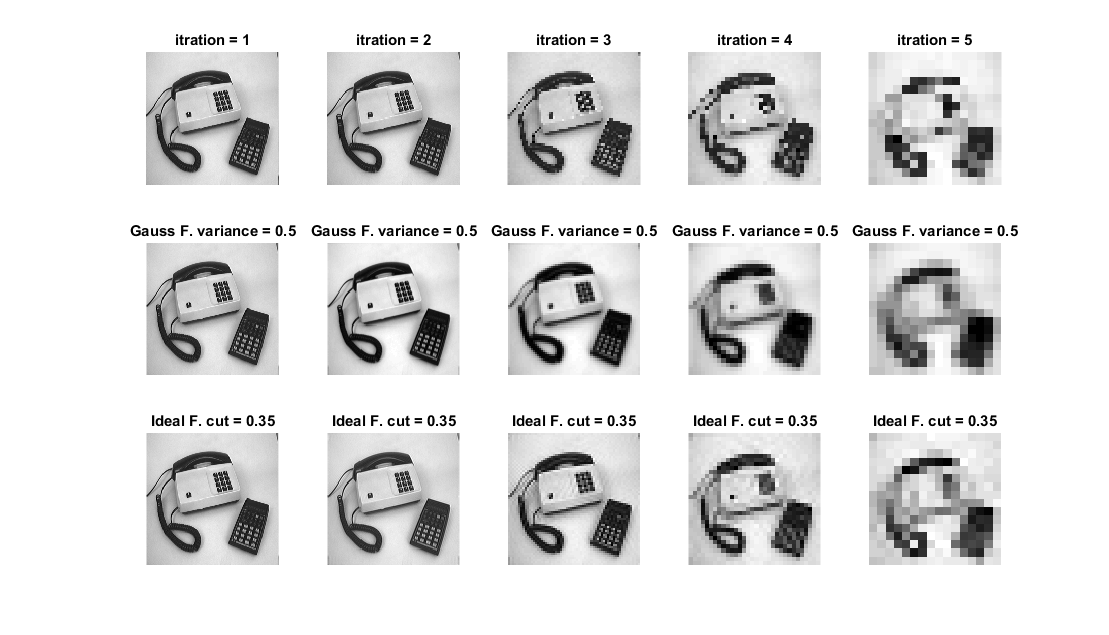
\includegraphics[width = \linewidth]{Lab1_3-2.png}
    \caption{Results of subsampling with smoothing by Gaussian and Ideal low pass filter in comparison to subsampling without smoothing.}
    \label{fig3_2}
\end{figure}


\item \textbf{What conclusions can you draw regarding the effects of smoothing when combined with subsampling? Hint: think in terms of frequencies and side effects.}

When we smooth an image we are reducing its highest frequency. This fact, added to what the sampling theorem states, makes the ``loss of information'' in the sampling be attenuated. What the sampling theorem states is that, if a signal is sampled at a rate equal or greater than twice its highest frequency, the original signal can be completely recovered from the samples. So smoothing the images makes the sampling process be less harmful, by means of decreasing the highest frequency.

\end{enumerate}

\end{document}